\lezione{5}{17.03.17}

\section{Costruzione di una probabilità}
L'obiettivo di questo capitolo è quello di definire una probabilità su un'algebra semplice e di mostrare, con l'aiuto di alcuni  teoremi, che la sua \emph{estensione} a una $\sigma$-algebra esiste ed è unica.
Da qui il concetto di \emph{costruzione} di una probabilità:
partendo da una collezione ristretta di eventi (come un'algebra), corrispondenti per esempio agli eventi verificabili sperimentalmente nel mondo reale, si è in grado di estendere le loro proprietà a una classe più ampia di eventi (come una $\sigma$-algebra).

\subsection{Estensione di una probabilità}

\medskip
Riformuliamo la definizione di probabilità su un'algebra invece che su una $\sigma$-algebra:\\[-8pt]
\begin{defn}
  \index{probabilità!su un'algebra}
  Siano $(\Omega, \Ac)$ spazio misurabile,
  $\Ac_0 \subseteq 2^\Omega$ algebra su $\Omega$.

  $\PP:\Ac_0 \to [0,1]$ è una probabilità se valgono le seguenti condizioni:
  \begin{enumerate}
    \item $\PP(\Omega) = 1$;
    \item $\PP$ è $\sigma$-additiva: dati $A_n \in \Ac_0 \ \forall n \in \NN$, allora:
      $$A_k \cap A_l  = \varnothing \enspace \forall k \neq l, \ \bigcup\limits_{n} A_n \in \Ac_0  \implies \PP\left(\bigcup\limits_{n} A_n \right) = \sum\limits_{n} \PP(A_n)$$
  \end{enumerate}
\end{defn}

\begin{teob}[\JPTh{6.1}]
  \label{teo-dalla-dimostrazione-ignota}
  Siano $\Omega$ spazio campionario, $\Ac_0$ algebra su $\Omega$, $\PP_0$ probabilità su $\Ac_0$. \\
  Allora $\exists!$ probabilità $\PP$ su $\Ac = \sigma(\Ac_0)$ che estende $\PP_0$, ovvero tale che:
  \begin{center}
  	$\PP(A) = \PP_0(A) \enspace \forall A \in \Ac_0$
  \end{center}
\end{teob}

Il teorema è un'immediata conseguenza del corollario \ref{coro-estensione-prob}, che introdurremo poco più avanti.

\medskip
\begin{defn}
  Una \textbf{collezione $\Cc \subseteq 2^\Omega$}:
  \begin{itemize}
    \item  è \textbf{chiusa per intersezioni finite} se: \index{chiusura!per intersezioni finite}
      $$A_1, \dots, A_n \in \Cc \implies \bigcap\limits_{k=1}^{n} A_k \in \Cc$$
    \item è \textbf{chiusa per limiti crescenti} se: \index{chiusura!per limiti crescenti}
      $$\{A_n\}_{n \in \NN} \subseteq \Cc, \enspace A_n \uparrow A \implies A \in \Cc$$
    \item è \textbf{chiusa per differenze} se: \index{chiusura!per differenze}
      $$ A,B \in \Cc, \enspace A \subseteq B \implies B \ \setminus \ A = B \cap A^C \in \Cc$$
  \end{itemize}
\end{defn}

\medskip
\begin{nb}
  Una $\sigma$-algebra è chiusa per intersezioni finite, limiti crescenti e differenze, mentre un'algebra è chiusa per intersezioni finite e differenze, ma in generale non per limiti crescenti.
\end{nb}

\subsubsection{Classi monotone e corollari}
\begin{teo}[classi monotone \JPTh{6.2}]\label{teo-classi-monotone}
  \index{classi monotone, teorema delle}
  Sia $\Cc \subseteq 2^\Omega$ chiusa per intersezioni finite, con $\Omega \in \Cc$. \\
  Sia inoltre $\Dc \subseteq 2^\Omega$ la più piccola collezione di insiemi tale che $\Dc \supseteq \Cc$, chiusa per limiti crescenti e per differenze. Allora:
  $$\Dc = \sigma(\Cc)$$
\end{teo}
Il teorema è anche noto come \emph{lemma di Dynkin}.

\medskip
\begin{dimo}
La dimostrazione si svolgerà secondo i seguenti punti:
\begin{enumerate}
  \item $\Dc$ esiste ed è ben definita;
  \item definizione della classe $\Dc_B$;
  \item $\Dc_B$ è chiusa per limiti crescenti;
  \item $\Dc_B$ è chiusa per differenze;
  \item $\Dc$ è chiusa per intersezioni finite particolari;
  \item $\Dc$ è chiusa per intersezioni finite;
  \item $\Dc$ è una $\sigma$-algebra;
  \item conclusione.

\end{enumerate}
\medskip
\begin{enumerate}
  \item Sia $\Dc_i$ (con $i \in I$) un gruppo di collezioni contenute in $2^\Omega$ che rispettano tutte le proprietà richieste a $\Dc$ nelle ipotesi (ovvero $\Dc_i \supseteq \Cc$ e $\Dc_i$ chiusa per limiti crescenti e per differenze, $\forall i$). Analizziamo le proprietà della loro intersezione $\Dc \coloneqq \bigcap_i \Dc_i$:
  \begin{enumerate}
    \item Sia $A \in \Cc$. Allora $A \in \Dc_i \enspace \forall i \implies A \in \Dc \implies \Dc \supseteq \Cc$.
    \item Siano $A_n \in \Dc \enspace \forall n \in \NN$, tali che $A_n \uparrow A$. Allora $ A_n \in \Dc_i \enspace \forall i \enspace \forall n \implies A = \bigcup_n A_n \in \Dc_i \enspace \forall i \implies A \in \Dc$
  Dunque $\Dc$ è chiusa per limiti crescenti.
    \item Sia $A \subseteq B$ con $A,B \in \Dc$. Allora $B \ \setminus \ A \subseteq A \in \Dc \implies B \ \setminus \ A \in \Dc$.
  \end{enumerate}
  Posso dunque prendere $\Dc = \bigcap_i \Dc_i$, che esiste e rispetta le tre proprietà richieste.
  \item Sia $B \in \Dc$ fissato arbitrariamente.
  Definiamo la seguente sottoclasse:
  $$ \Dc_B \coloneqq \left \{ A \in \Dc: \ A \cap B \in \Dc \right \}$$
  Notiamo che $\Dc_B \subseteq \Dc$.
  \item Siano $A_n \in \Dc_B \enspace \forall n$ tali che $A_n \uparrow A$.
  Poiché $A_n \in \Dc_B \subseteq \Dc$, allora $A_n \in \Dc$. Ma essendo $\Dc$ chiusa per limiti crescenti, $A \in \Dc$. Inoltre:
  $$A \cap B = \left(\bigcup_n A_n\right) \cap B = \bigcup_n(A_n \cap B) \in \Dc$$
  Perché $\Dc$ è chiusa per limiti crescenti. \\
  Dunque $A \in \Dc_B$ per definizione di $\Dc_B$: in altre parole, $\Dc_B$ è chiusa per limiti crescenti.

  \item Siano $A_1, \, A_2 \in \Dc_B$ tali che $A_1 \subseteq A_2$. \\
  $A_2 \, \setminus \, A_1 \in \Dc$, perché $A_2 \in \Dc_B \subseteq \Dc, \ A_1 \in \Dc_B \subseteq \Dc \ $ e $\Dc$ è chiusa per differenze.
  Inoltre:
  $$(A_2 \, \setminus \, A_1) \cap B = (A_2 \cap A_1^C) \cap B = (A_2 \cap B) \, \setminus \, (A_1 \cap B) \implies (A_2 \, \setminus \, A_1) \cap B \in \Dc$$
  Quindi entrambi gli insiemi appartengono a $\Dc_B \subseteq \Dc$, la quale è chiusa per differenze.
  Pertanto, $(A_2 \, \setminus \, A_1) \in \Dc_B$ per definizione di $\Dc_B$, ovvero $\Dc_B$ è chiusa per differenze.
  \item Dimostriamo ora che $\Dc = \Dc_C \enspace \forall C \in \Cc$, ovvero che $\Dc$ è chiusa per intersezioni del tipo $D \, \cap \, C$, con $D \in \Dc$ e $C \in \Cc$. \\
  Sia $A \in \Cc$. Per definizione di $\Dc$, $A \in \Dc$; inoltre $C \in \Cc \subseteq \Dc$. Allora $A \cap C \in \Dc$, e di conseguenza $A \in \Dc_C$ per definizione di $\Dc_C$.
  Poiché $A$ è un generico elemento di $\Cc$, troviamo che $\Cc \subseteq \Dc_C$, e come già sappiamo, $\Dc_C \subseteq \Dc$. $\Dc_C$ rispetta le tre proprietà richieste per $\Dc$ ($\Dc_C \subseteq \Cc$, chiusura per limiti crescenti e differenze). Ma allora deve essere $\Dc_C = \Dc$.

  \item Sia $A \in \Cc$. Per definizione di $\Dc$, $A \in \Dc$; inoltre per il punto precedente $A \cap B \in \Dc$; ma allora $A \in \Dc_B$. Ciò significa che $\Cc \subseteq \Dc_B \subseteq \Dc$. Ma $\Dc_C$ rispetta le tre proprietà di $\Dc$, e dunque deve essere $\Dc_C = \Dc$.
  \item Verifichiamo le tre proprietà caratteristiche delle $\sigma$-algebre:
  \begin{enumerate}
    \item $\Omega \in \Dc$, poiché $\Omega \in \Cc$ per ipotesi, e $\Cc \in \Dc$. $\varnothing \in \Dc$, poiché $\varnothing = \Omega \ \setminus \ \Omega$ e $\Dc$ è chiusa per differenze.
    \item $ A \in \Dc \implies A^C = \Omega \ \setminus \ A \in \Dc$, poiché $\Dc$ è chiusa per differenze.
    \item ($\sigma$-additività) Siano $ A_n \in \Dc \enspace \forall n \in \NN.$ \\
    Dopo aver definito la successione crescente $B_k = \bigcup_{n=1}^{k} A_n$, abbiamo che $\bigcup_n A_n = \bigcup_k B_k$.
    Ma $ B_k \in \Dc$, poiché:
    $$B_k = \bigcup_{n=1}^k A_n = \left( \bigcap_{n=1}^k A_n^C \right)^C$$
    e $\Dc$ è chiusa per intersezioni finite. \\
    Abbiamo poi che:
    $$B_k \, \uparrow \, \bigcup_{k=1}^{{+\infty}} B_k = \bigcup_{n=1}^{{+\infty}} A_n$$
    Questa unione appartiene a $\Dc$ poiché esso è chiuso per limiti crescenti.
    È dunque dimostrata la chiusura per unione numerabile; quella per intersezione numerabile si dimostra in maniera analoga.
  \end{enumerate}
  $\Dc$ è dunque una $\sigma$-algebra.
  \item $\Dc$ deve per forza coincidere con $\sigma(\Cc)$: infatti, se $\Dc$ è una $\sigma$-algebra, allora $\Dc \supseteq \sigma(\Cc)$ per definizione di $\sigma(\Cc)$ e $ \Dc \subseteq \sigma(\Cc)$ per definizione di $\Dc$. \qedhere
  \end{enumerate}
\end{dimo}

\medskip
\begin{coro}\label{coro-estensione-prob}
  Siano $(\Omega, \Ac)$ spazio misurabile, $\PP$ e $\QQ$ probabilità su $\Ac$, e $\Cc \subseteq \Ac$ classe chiusa per intersezioni finite e tale che $\sigma(\Cc) = \Ac$.
  Se $\PP(A) = \QQ(A) \enspace \forall A \in \Cc$ (ovvero, usando una notazione alternativa, $\PP\big|_{\Cc} = \QQ\big|_{\Cc}$), allora $\PP(A) = \QQ(A) \enspace \forall A \in \Ac$, ovvero $\PP \equiv \QQ$.
\end{coro}
In altre parole, è garantita l'\emph{unicità dell'estensione} di una probabilità su una classe che rispetti le opportune ipotesi: se i valori di $\PP$ e $\QQ$ coincidono sugli insiemi della suddetta classe (la quale è un sottoinsieme del dominio), allora coincideranno anche su tutto il dominio $\Ac$, ovvero le due probabilità devono necessariamente essere la stessa.

\begin{dimo}
  Sia $\widetilde{\Cc} = \Cc \cup \{\Omega\}$ che è ovviamente chiusa per intersezioni finite. Si definisca ora:
  $$\widetilde{\Dc} \coloneqq \left \{ A \in \Ac: \PP(A) = \QQ(A) \right \}$$
  \leavevmode
  \begin{enumerate}
    \item $\widetilde{\Dc} \supseteq \widetilde{\Cc}$ perché $\widetilde{\Dc} \supseteq \Cc$ per ipotesi e $\Omega \in \widetilde{\Dc}$ in quanto $\PP( \Omega) = 1 = \QQ(\Omega)$.
    \item Siano $A_n \in \widetilde{\Dc} \enspace \forall n$, con $A_n \uparrow A$. Allora $\PP(A_n) = \QQ(A_n) \ \forall n$. Prendendo il limite per $n \to +\infty$ di entrambi i membri, $\PP(A) = \QQ(A) \implies A \in \widetilde{\Dc}$. Ergo, $\widetilde{\Dc}$ è chiusa per limiti crescenti.
    \item Siano $A, B \in \widetilde{\Dc}$ tali che $A \subseteq B$. Allora:
    $$\PP( B \ \setminus \ A) = \PP(B) - \PP(A) = \QQ(B) -\QQ(A) = \QQ( B \ \setminus \ A) \implies B \ \setminus \ A \in \widetilde{\Dc}$$
    Quindi  $\widetilde{\Dc}$ è chiusa per differenze.
  \end{enumerate}
  Grazie a queste 3 proprietà è possibile invocare il teorema delle classi monotone: $\widetilde{\Dc} \supseteq \sigma(\widetilde{\Cc})$. Il segno di inclusione è necessario in quanto sappiamo che $\widetilde{\Dc}$ rispetta le 3 proprietà, ma non è detto che sia essa stessa la classe più piccola che le soddisfa, ovvero $\sigma(\widetilde{\Cc})$: in ogni caso la prima contiene sicuramente la seconda. Ora, poiché $\sigma(\widetilde{\Cc}) = \sigma(\Cc) = \Ac$, si ottiene che $\PP(A) = \QQ(A) \ \forall A \in \Ac$. \qedhere
\end{dimo}

\medskip
\begin{coro}[criterio di Caratheodory]
  Siano $\Omega$ spazio campionario, $\Ac_0$ algebra su $\Omega$, $\Ac = \sigma(\Ac_0)$, $\PP$ e $\QQ$ probabilità su $\Ac$.
  Se $\PP(A) = \QQ(A) \ \ \forall A \in \Ac_0$, allora $\PP(A) = \QQ(A) \ \ \forall A \in \Ac$.
\end{coro}
Questo è un'immediata conseguenza del corollario precedente (\ref{coro-estensione-prob}) per il fatto che qualsiasi algebra è, per definizione, chiusa per intersezioni finite.
A parte questa minima variazione nelle ipotesi, i due corollari sono identici: quest'ultimo afferma che l'\emph{estensione di una probabilità da un'algebra alla corrispondente $\sigma$-algebra è unica}.
È dunque sufficiente essere in possesso di un'informazione su un ristretto gruppo di insiemi (due probabilità sono identiche su un'algebra) per poter affermare una proprietà generale dell'intera $\sigma$-algebra generata (esse sono identiche su tutto il dominio).

\medskip
\begin{cese}
  Mostriamo che l'ipotesi della \emph{chiusura} di $\Cc$ \emph{per intersezioni finite} è essenziale per l'applicazione dei corollari mediante un controesempio in cui questa ipotesi è mancante. \\*
  Considerando una $\Omega$ qualsiasi e delle sue partizioni $A_1, A_2, B_1, B_2$ e dati $\Ac = \sigma(A_1, A_2, B_1, B_2)$,
  $\PP$ e $\QQ$ probabilità su $\Ac$, si ha: \\*
  $$\PP(A_k) = \frac{1}{4} + \frac{1}{4} = \frac{1}{2} \stackrel{\downarrow}{=} \frac{1}{2} + 0 = \QQ(A_k) \quad \forall k = 1, 2$$
  \begin{figure}[H]
    \centering
    \def\drect {(0,0) rectangle (3,2)}
    \def\prect {(0,0) rectangle (1.5,1)}
    \def\srect {(1.5,0) rectangle (3,1)}
    \def\trect {(0,1) rectangle (1.5,2)}
    \def\qrect {(1.5,1) rectangle (3,2)}

    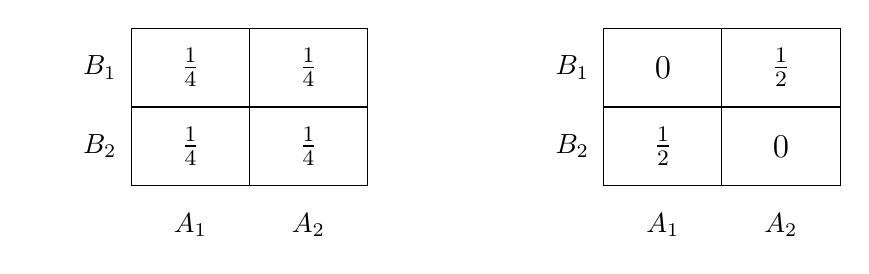
\begin{tikzpicture}
      \begin{scope}
        \draw \drect node[pos=0, yshift=1.0cm, xshift=-1.2cm] {\huge $\PP$};
        \draw \prect node[pos=.5] {\large $\frac{1}{4}$};
        \draw \srect node[pos=.5] {\large $\frac{1}{4}$};
        \draw \trect node[pos=.5] {\large $\frac{1}{4}$};
        \draw \qrect node[pos=.5] {\large $\frac{1}{4}$};
        \node at (-0.4, 1.5) {$B_1$};
        \node at (-0.4, 0.5) {$B_2$};
        \node at (0.75, -0.5) {$A_1$};
        \node at (2.25, -0.5) {$A_2$};
      \end{scope}

      \begin{scope}[shift={(6cm,0cm)}]
        \draw \drect node[pos=0, yshift=1.0cm, xshift=-1.2cm] {\huge $\QQ$};
        \draw \prect node[pos=.5] {\large $\frac{1}{2}$};
        \draw \srect node[pos=.5] {\large $0$};
        \draw \trect node[pos=.5] {\large $0$};
        \draw \qrect node[pos=.5] {\large $\frac{1}{2}$};
        \node at (-0.4, 1.5) {$B_1$};
        \node at (-0.4, 0.5) {$B_2$};
        \node at (0.75, -0.5) {$A_1$};
        \node at (2.25, -0.5) {$A_2$};
      \end{scope}
    \end{tikzpicture}
  \end{figure}
  In questo caso dunque si può effettivamente affermare che $\PP(A) = \QQ(A) \ \forall A \in \Cc$ e che $\PP(B) = \QQ(B) \ \forall B \in \Cc$, ma il corollario alle classi monotone è inapplicabile perché $\Cc$ non è chiusa per intersezioni finite (come richiesto dalle ipotesi): per esempio $A_1 \cap B_2 \notin \Cc$.
  Infatti in questo caso si può facilmente verificare che $\PP \centernot\equiv \QQ$.
\end{cese}

\medskip
\begin{nb}
  Possono esistere esperimenti diversi che hanno la stessa probabilità, il fatto che $\PP: \Ac \to [0,1]$ sia uguale non garantisce che per ogni esito elementare la probabilità sia uguale.
\end{nb}
\begin{ese}[lancio di due dadi]
  Preso un d8\footnote{Ovvero ``dado a 8 facce'', per i tre lettori che non sanno cosa siano i giochi di ruolo.} non truccato, si consideri la $\sigma$-algebra $\Ac = \{\emptyset$, pari, dispari, $\Omega\}$, di conseguenza la probabilità $\PP$ è:
  \begin{table}[H]
    \def\arraystretch{1.5}
    \centering
    \begin{tabular}{|c|c|c|c|c|}
    \hline
    $\Ac$ & $\emptyset$ & pari & dispari & $\Omega$ \\ \hline
    $\PP$ & $0$ & $\frac{1}{2}$ & $\frac{1}{2}$ & $1$ \\ \hline
    \end{tabular}
  \end{table}
  Si consideri un secondo d8, truccato, in cui escono uniformemente solo gli esiti da 1 a 4, mentre gli altri hanno probabilità zero. Scegliendo la stessa $\sigma$-algebra si ottiene la probabilità $\QQ$ che è identica a $\PP$.

  Nonostante i due esperimenti abbiano esiti elementari $\omega$ diversi, la probabilità è uguale perché questa non dipende direttamente da $\Omega$.
\end{ese}

%\textit{NdR: in questa lezione è stata svolta la costruzione di una probabilità su $\Omega = \RR$, ma nella lezione successiva è stata ri-enunciata e ri-dimostrata in maniera più compatta nel teorema \ref{teo-prob-ripartizione}, quindi è stato scelto di ometterla qui.}

\esercitazione{4}{21.03.17}
\subsection{Probabilità su spazi finiti e discreti}
\begin{defn}
  Sia dato uno spazio probabilistico $(\Omega,\Ac,\PP)$ in cui:
  \begin{itemize}
    \item $\Omega$ è uno spazio campionario finito e discreto tale che $\#\Omega = n$;
    \item $\Ac$ è la $\sigma$-algebra definita su $\Omega$ come $\Ac = 2^{\Omega}$;
    \item $\PP$ è la probabilità costruita sulla $\sigma$-algebra $\Ac$ definita come:
    $$\PP(\{\omega\})=\frac{1}{\#\Omega} \text{ e con } \PP(\{A\})=\frac{\#A}{\#\Omega}.$$
  \end{itemize}
  Tale spazio probabilistico si dice \textbf{spazio probabilistico discreto e uniforme}, cioè lo spazio è discreto, finito e tutti gli esiti sono equiprobabili.
\end{defn}
%Si rimanda all'appendice A, a pagina \pageref{appendice-combinatorio}, per la trattazione relativa al calcolo combinatorio.
\cleardoublepage
